\chapter{Scramble Services Implementation}
\label{ch:WP}

\section{Translator}
\paragraph{}
In a hierarchical architecture involving different MANOs, there is a need of conversion of network descriptors to schemas of respective MANO. Service Descriptor Translator (SDT) serves the purpose of translating network descriptors, namely NSDs and VNFDs from schema of SONATA Pishahang to that of OSM and vice versa.
\paragraph{}
In a scenario, where a parent MANO, say Pishahang decides to deploy one of the network services in its lower hierarchy MANO, say OSM, the NSD and VNFD(s) need to be converted to the descriptor schema of OSM. In such an event, the Scramble plugin calls the translator service and sends the descriptors to the SDT, where the translation of the descriptors takes place and the translated descriptors are sent to Adaptor utility for deployment in appropriate MANO. 


\subsection{Architecture \& Work flow}
The translator engine reads a json formatted descriptor and first converts it into a pandas \textit{DataFrame}. The \textit{DataFrame} object is constructed to have the following columns.

\begin{table}[H]
	\begin{center}
		\caption{Descriptor represented DataFrame.}
		\label{tab:table1}
		\begin{tabular}{l|l} 
			\textbf{Columns} & \textbf{Description} \\
			\hline
			\textbf{parent\_level} & It stores immediate parent key's depth-level \\ 
			\textbf{parent\_key} & It stores immediate parent key  \\
			\textbf{level} & It stores current key's depth-level \\
			\textbf{key} & It stores current key \\
			\textbf{value} & It stores current key's value \\
			\textbf{lineage} & \makecell[l]{It stores current key's entire lineage from the root depth-level.\\ It is useful to store the nested information} \\  
		\end{tabular}
	\end{center}
\end{table}

The \textit{setup} and \textit{transformation} classes of the translator engine carries out all the transformation, needed to translate between OSM and Pishahang descriptors, on the \textit{DataFrame} object. Once all the transformation are over, the resulting \textit{DataFrame} is then converted again into a json (refer Figure  \ref{fig:sequence-diagram-translator}).

\begin{figure}[h!]
	\centering
	\includegraphics[width=1\linewidth]{"figures/translator_seq_diag"}
	\caption{Translator sequence diagram}
	\label{fig:sequence-diagram-translator}
\end{figure}


\subsection{Modules}
The Translator engine consists of the following modules (refer Figure  \ref{fig:class-diagram-translator}):
\begin{enumerate}
	\item descriptorReader
	\subitem class: read\_dict
	\item descriptorWriter
	\subitem class: write\_dict
	\item utilities
	\subitem class: setup
	\subitem class: transformation
	\subitem class: insert\_into\_db
	\item translator
	\subitem class: TranslatorService
	\item validator
	
\end{enumerate}

\begin{figure}[h!]
	\centering
	\includegraphics[width=1\linewidth]{"figures/class_diagram_translator"}
	\caption{Translator class diagram}
	\label{fig:class-diagram-translator}
\end{figure}



\subsubsection{descriptorReader}
The class \textit{read\_dict} is responsible to read a json/dictionary input (NSD/VNFD) and iterate over the keys and return a generator of an object to the calling program. This generator can be transformed to any python data structure for ease of use and navigation. 

The input to this module is a json or dictionary object.

\begin{lstlisting}[language=Python,caption=reader to read a json into a DataFrame, label=lis:descriptorReader]
from descriptorReader import read_dict

pishahang = pishahang_descriptor ## the descriptor as a json or dict object

### reading a dict/ json content into a pandas dataframe
reader = read_dict()

pishahang_dataset = pd.DataFrame(
reader.dict_parser(pishahang,'root', 1, '0|preroot|0'), 
columns=['parent_level', 'parent_key', 'level', 'key', 'value', 'lineage'])


pishahang_dataset.sort_values(ascending=True, by=['level', 'parent_key'],inplace=True)
pishahang_dataset.fillna('NULL', inplace=True)
pishahang_dataset.reset_index(drop=True,inplace=True)

\end{lstlisting}
\subsubsection{descriptorWriter}

The class \textit{write\_dict} is responsible to read a python pandas Dataframe input and output a nested json/dictionary maintaining the nested structure in the dictionary.

\begin{lstlisting}[language=Python,caption=writer to write a translated DataFrame into a json, label=lis:descriptorWriter]
from descriptorWriter import write_dict

### writing from a pandas dataframe to a dict/json object
writer = write_dict()
pishahang_descriptor = writer.translate(pishahang_dataset.sort_values(by='lineage'))

\end{lstlisting}

\subsubsection{utilities}

The class \textit{setup} is responsible for transforming the keys and map the corresponding values between sonata and osm descriptors. The class includes 4 functions for translating between sonata and OSM descriptors. 
\begin{enumerate}
	\item translate\_to\_osm\_nsd()
	\item translate\_to\_osm\_vnfd()
	\item translate\_to\_sonata\_nsd()
	\item translate\_to\_sonata\_vnfd()
\end{enumerate}

The class \textit{transformation} acts as a helper class for the task of transforming the dataframe between sonata and OSM structures. 

\subsubsection{translator}

The class \textit{TranslatorService} is the interface where the actual translation request comes in. After a tranlsation request is received along with a descriptor, it calls the above modules translate and validate the descriptors (NSD/VNFD).

This following function translates OSM descriptor to Pishahang and vise-versa.
\begin{lstlisting}[language=Python,caption= Translating descriptor between Pishahang and OSM, label=lis:toSOnata]
import pymongo
from validate import validator
from utilities import setup


class TranslatorService():

def __init__(self,client = pymongo.MongoClient("mongodb://mongo:27017")):
self.setup_obj = setup(client)
self.validate_obj = validator()


def toSonata(self,received_file):

if 'vnfd:vnfd-catalog' in received_file:

doc = self.setup_obj.db_descriptors["translated_vnfd"]
translated = self.setup_obj.translate_to_sonata_vnfd(received_file)

check = self.validate_obj.sonata_vnfd_validate(translated)

if check == "True":
temp = doc.insert_one(translated)
translated_ref = temp.inserted_id

elif 'nsd:nsd-catalog' in received_file:

doc = self.setup_obj.db_descriptors["translated_nsd"]
translated = self.setup_obj.translate_to_sonata_nsd(received_file)

check = self.validate_obj.sonata_nsd_validate(translated)

if check == "True":
temp = doc.insert_one(translated)
translated_ref = temp.inserted_id

return {"descriptor":translated ,"VALIDATE STATUS" :check}

def toOsm(self,received_file):

if 'network_functions' in received_file:

doc = self.setup_obj.db_descriptors["translated_nsd"]
translated = self.setup_obj.translate_to_osm_nsd(received_file)

check= self.validate_obj.osm_validator(translated)

if check == "True":
temp = doc.insert_one(translated)
translated_ref = temp.inserted_id

elif 'virtual_deployment_units' in received_file:

doc = self.setup_obj.db_descriptors["translated_vnfd"]
translated = self.setup_obj.translate_to_osm_vnfd(received_file)

check= self.validate_obj.osm_validator(translated)

if check == "True":
temp = doc.insert_one(translated)
translated_ref = temp.inserted_id

return {"descriptor":translated ,"VALIDATE STATUS" :check}
\end{lstlisting}

\subsubsection{validator}

The validator validates the descriptors presented for translation. The simplest form of validation of the descriptors begins with validating the syntax of the given descriptors, implemented using python library called \textit{jsonschema.draft4validator}, this library compares the given descriptor with corresponding schema provided and if errors are found then the error and the path of the error is printed. This error path is handy and is important, as a typical descriptor has many keys with identical names.

The function in appendix \ref{tvalidation} validates the syntax of provided and translated OSM and Sonata descriptors with its corresponding schemas.

 The next stage of validation is checking the semantics of the descriptors, for Sonata this is achieved by validating the Integrity of the given descriptors.
 \begin{enumerate}
 	\item Integrity Validation: For validation of integrity of a NSD the corresponding VNFD's are required, which then checks the connection points and virtual links in NSD and VNFD's. If there is a correlations between the connection points and virtual links in NSD and VNFD's then the validation holds true.
 	
 	\begin{enumerate}
 		\item The Function def \textit{sonata\_nsd\_validate(self,descriptor, vnfd = None)}, accepts NSD and its corresponding zero or more VNFD's. If one or more VNFD's are provided the the integrity and topology validation occurs else just the syntax is checked.  
 	\end{enumerate}
 	   
 \end{enumerate}
 
 For checking the semantics of the OSM descriptors, python object class which is generated from the .Yang files provided by OSM. The provided descriptors are then passed as parameters to this python object class with the help of python library called \textit{pybindJSONDecoder.load\_ietf\_json()}. The resulting output will be true if successfully validated else the error in the descriptor is given.
 
 \begin{enumerate}
 	\item In the class \textit{def osm\_validator(self,descriptor)}, the descriptor in the form of python dictionary is taken as input and syntax is checked first, later the descriptor is passed to class "osm\_dep\_validator(descriptor\_to\_validate)" to check semantics.
 	
 	\item in class \textit{osm\_dep\_validator(descriptor\_to\_validate)}, \textit{pybindJSONDecoder.load\_ietf\_json(data, None, None, obj=mynsd)} is used where data is the given descriptor, obj is the Python object class in file osmdata.
 \end{enumerate}

And thus a descriptor which is validated true is not only error free but also will be for sure accepted by Sonata, Pishahang and OSM as a valid descriptor. 

\subsection{Challenges}
\begin{enumerate}
	\item The initial challenges faced while designing the translator was mapping the "\textit{required}" keys between OSM and Pishahang descriptors. Figuring out the common functionalities of the respective "\textit{required}" keys in OSM and Pishahang was the priority and a mapping was created. The other "\textit{optional}" keys which were exclusive for each MANOs were also identified and sidelined for future work.
	\item The challenging part for the development of validator was for OSM. Currently available validator for OSM, is a package developed based on python object code and the problem is that only the error is printed. For example: if a error is found in key "ID", then the error message would be "invalid ID" and a typical descriptor contains multiple "ID" keys and it would be hard to find where exactly the error lies. Hence using various Python libraries a Json schema for OSM was developed with which not just the error but the exact path of the error is also given. 
\end{enumerate}

\subsection{Usage}

The class \textit{TranslatorService} takes input of two simple requirements.
\begin{enumerate}
	\item The first input is a descriptor in the form of json file or a python dictionary. The descriptor can be Pishahang or OSM.
	\item The second input is a parameter to let the translator know how the translation should take place. The parameters are
	  \begin{enumerate}
	  	\item \textit{osm\_to\_sonata} for translation of OSM descriptor to Pishahang.
	  	\item \textit{sonata\_to\_OSM} for translation of Pishahang descriptor to OSM.
	  \end{enumerate}
\end{enumerate}

The output will be a valid translated descriptor in the form of python dictionary.

\subsection{Future Work}	

Translator engine currently does not support the following:
\begin{enumerate}
	\item Forwarding Graph
	\item Juju charms in OSM
	\item Monitoring Parameters
\end{enumerate}

\subsubsection{Forwarding Graph}
Although translation of forwarding graphs between OSM and  Pishahang has been implemented, we could not verify the translation as the forwarding graph logic was not currently feasible during our implementation period in both OSM and Pishahang.

\subsubsection{Juju charms in OSM}
MANOs provide programmable and flexible management and orchestration of VNFs. OSM provides this flexibility through juju charms and Pishahang provides this through SSM/FSM (a container based solution). Because of these technological differences, direct translation between juju charms in OSM, and SSM (Service Specific Manager) and FSM (Function Specific Manager) in Pishahang is not possible. 

As an alternative, it is possible to add charms functionality to Pishahang so that a descriptor containing juju charms can be deployed in both Pishahang and OSM with direct translation. This can be achieved by adding or modifying below things in Pishahang.
\begin{enumerate}
	\item Modify packaging and unpackaging techniques in Pishahang to accept charm package along with descriptors
	\item Add additional keys in descriptors to mention charm name, actions and vnf index similar to OSM
	\item Update Pishahang installation code to install juju and charm programs and tools
	\item Create an interface to execute actions on VNFs
	\item Create new container or component to perform actions on specified VNFs
	\item Manage removal or deletion of charms after life cycle of Network Service 
\end{enumerate} 


\subsubsection{Monitoring Parameters}
Translation could be extended to include the monitoring parameters as well. However verifying monitoring parameters were not feasible in OSM during our implementation period, so we sidelined for future scope.

\newpage

\section{Splitter}
Splitter helps in splitting a Network Service (NS) into multiple sub Network services which can be deployed and instantiated individually on Internet Service Providers (ISPs) located over a vast geographical region spanning multiple domains and are orchestrated by different MANO frameworks. Splitter calls Service Descriptor Transltor if there is a need to translate the NS if it is to be deployed on a different MANO framework. In this work package, a Service Descriptor Splitter (SDS) is implemented which splits the NSD of a network service. SDS takes NSD as an input that contains all the information elements which can be extracted to generate separate NSDs. In the proposed approach, the service graph is extracted from the input NSD and is split into subgraphs that result in a separate NSD which includes a set of elements such as VNFs, Virtual Links (VLs), forwarding graphs of VNFs etc, according to the specific MANO framework.

\subsection{Architecture & Work flow}

Figure \ref{fig:osmschemaclassdiagram}, \ref{fig:osmsplitterclassdiagram}, \ref{fig:pishahangschemaclassdiagram} and \ref{fig:pishahangsplitterclassdiagram} represents class diagrams of OSM and Pishahang. Python base classes are used for different sections of a NSD which encapsulate all the attributes and its values into a single unit which makes it very easy to process. Once the objects are set they are passed to different splitting functions based on there type. We have two different processing units for OSM and SONATA. Figure \ref{fig:splittersequencediagram} shows the sequence diagram of Pishahang splitter. Following are some functions responsible for splitting the NSD.

\begin{itemize}
	\item \textbf{Validate: }Validation of the incoming request from MANO for splitting happens is done before actual splitting. Validation checks if the request has correct VNF ids. It also checks if the list of VNFs specified in the request is matching with the list of VNFs in the original NSD file.
	\item \textbf{Set connection point reference for virtual functions:}After validation, as per the incoming request multiple set of empty NSD objects are created. This step updates the empty NSD objects with connection points. These connection points are either of type “external” or “management”. Each sub NSD will have its own connection points just like its parent NSD.
	\item \textbf{Split Network Functions: }After creating connection points for each sub NSDs, VNF objects are set in the updated NSD objects as per the request from MANO. Each set of VNFs from the request is set in each of the NSD objects. 
	\item \textbf{Split Virtual Links: }When a NSD is splitted into different parts, its topology changes. Change in topology results in changing of Virtual Links. For example if A, B and C are three Nfs and we are splitting them in such a way so that A and B remain in one NSD and C in separate NSD. A virtual link between B and C now does not make sense. So this link should be broken down and B’s output should be connected to the external end point which was connected to C’s input earlier. This function splits these kind of Virtual Links.
	\item \textbf{Split Forwarding Graph: }Once the topology changes, the respective Forwarding graph also changes. Split forwarding graph pulls out the set of connection points and newly created virtual links and sets them in the sub NSDs. The current implementation can split a NSD with three or less VNFs. To maintain the topology of the original NSD, Splitter needs to extract virtual links from the main NSD and create new virtual links for sub NSDs in such a way that the topology of the main NSD is maintained. 
	\item \textbf{Create Sub-NSDs: } The last step is to return the sub-nsds created out of NSD objects.
\end{itemize} 

\begin{figure}
	\centering
	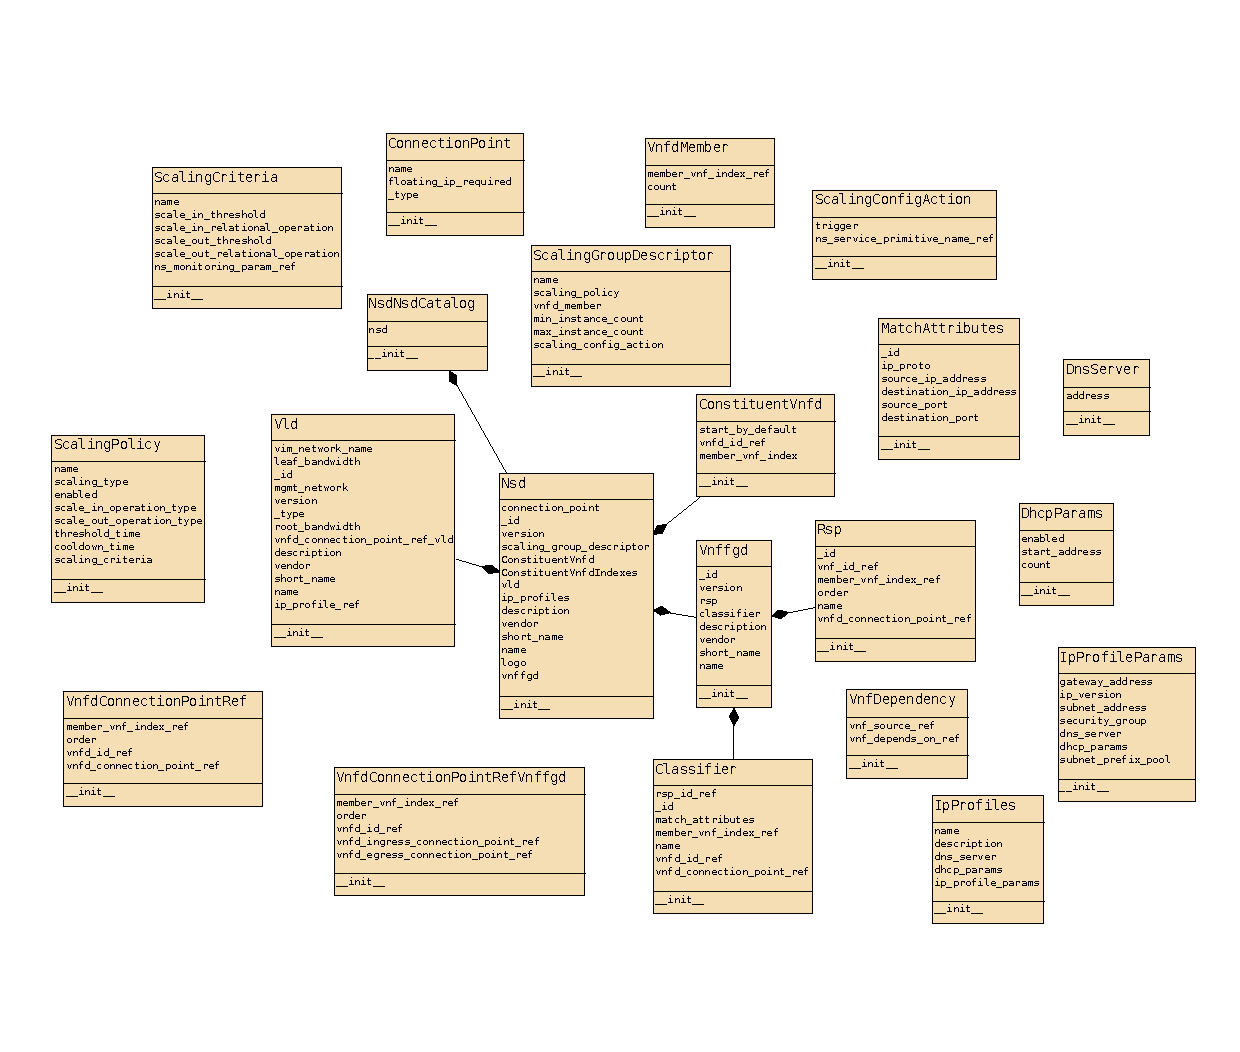
\includegraphics[width=1\linewidth]{figures/osm-schema}
	\caption{OSM Schema Class Diagram}
	\label{fig:osmschemaclassdiagram}
\end{figure}

\begin{figure}
	\centering
	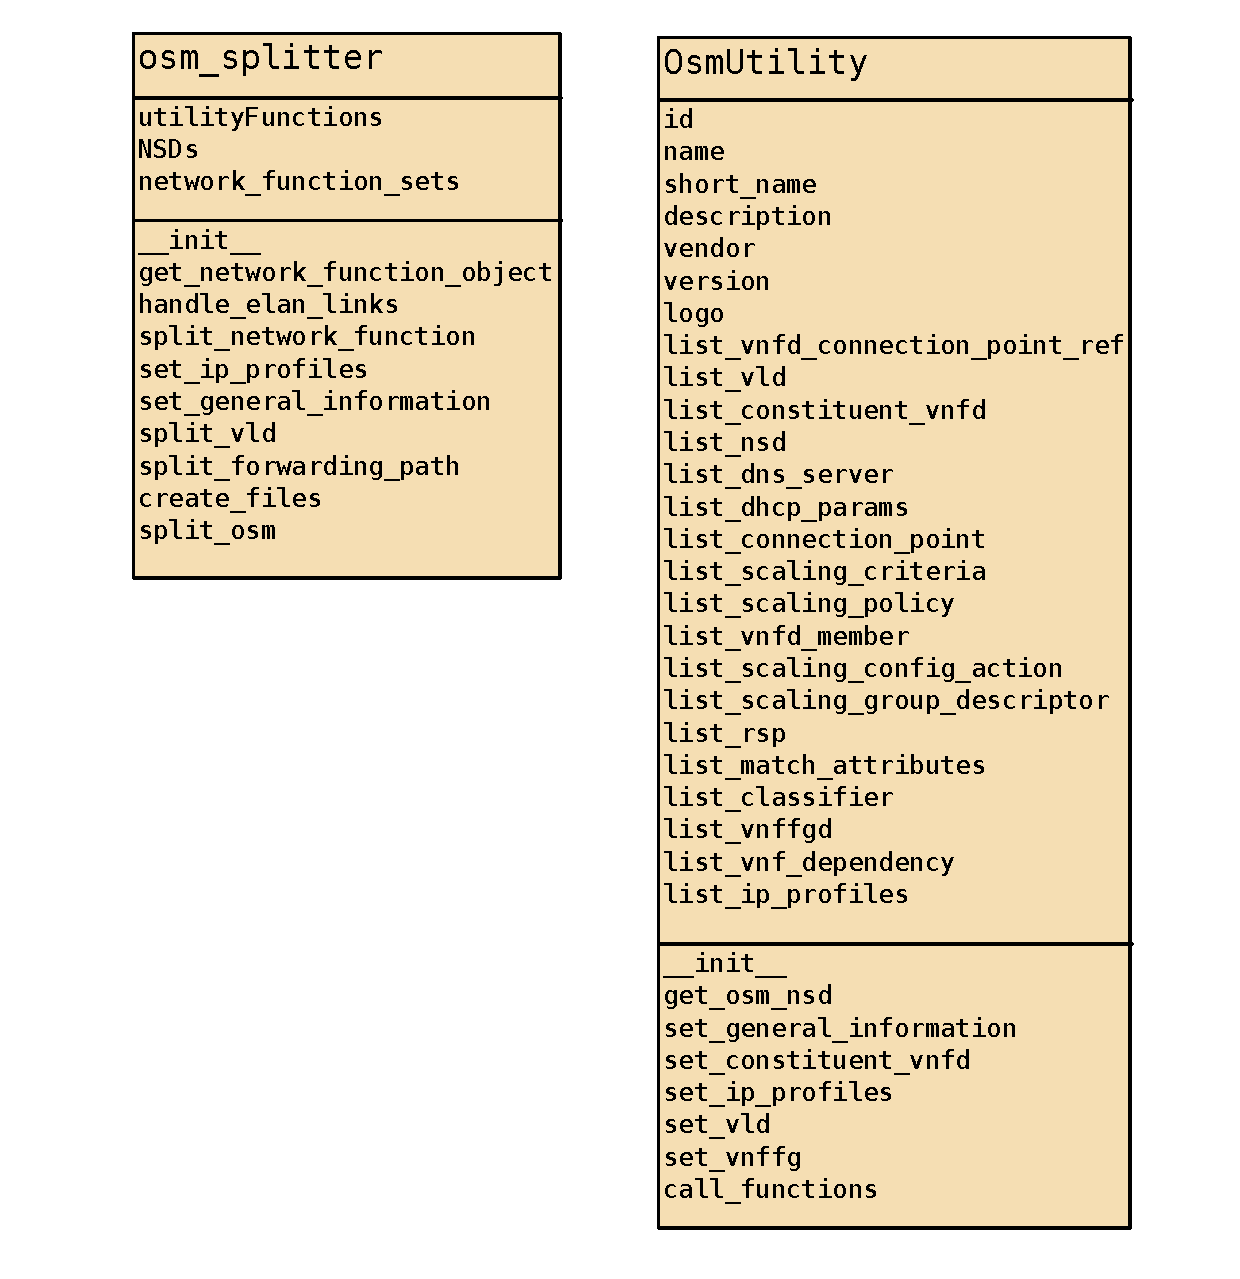
\includegraphics[width=1\linewidth]{figures/OSM-Splitter}
	\caption{OSM Splitter Class diagram}
	\label{fig:osmsplitterclassdiagram}
\end{figure}

\begin{figure}
	\centering
	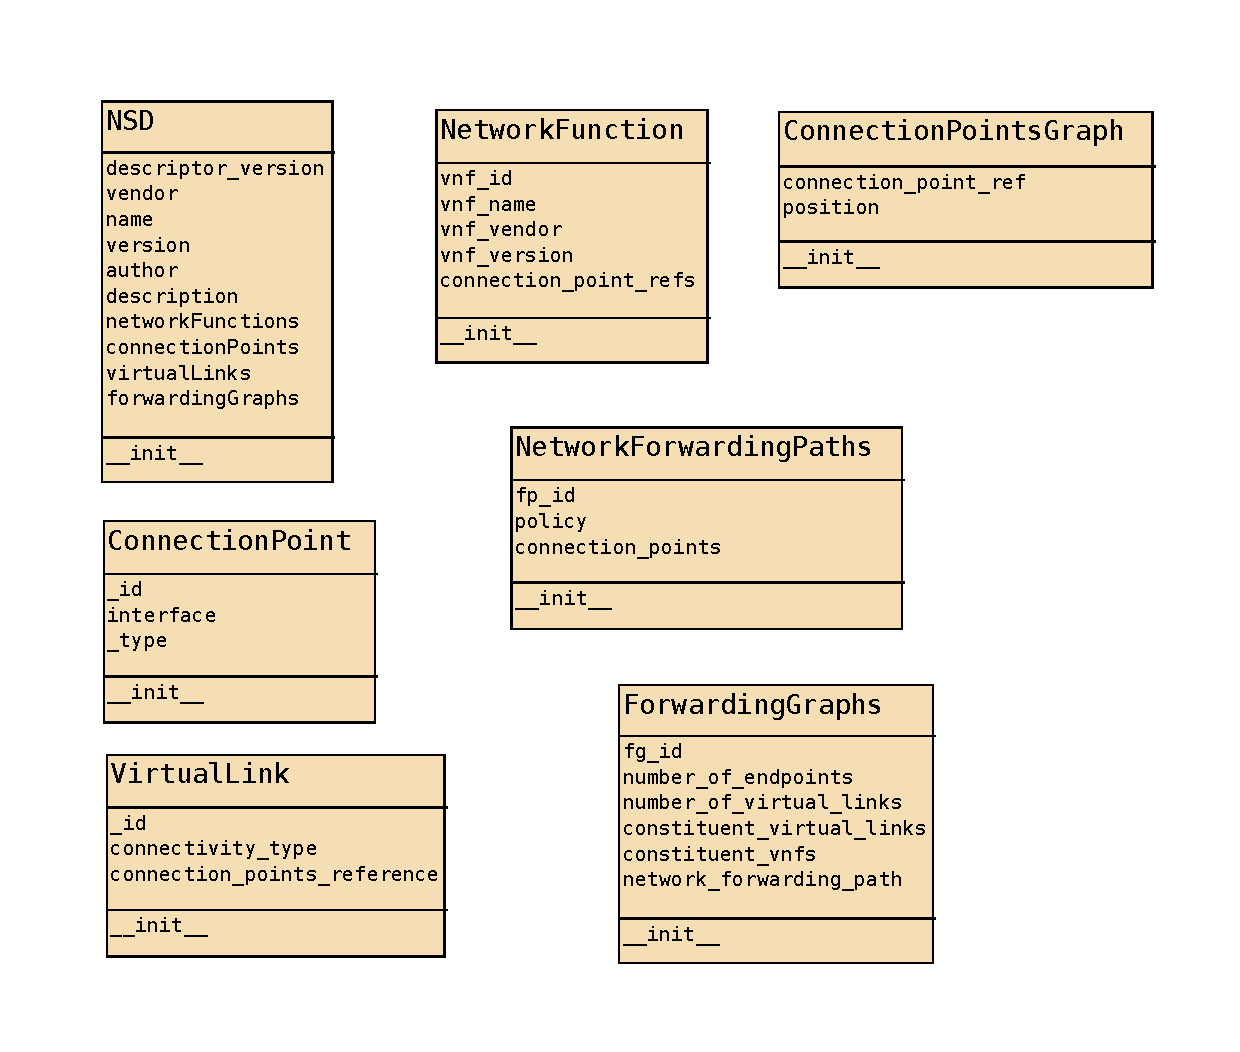
\includegraphics[width=1\linewidth]{figures/pishahang-schema}
	\caption{Pishahang Schema Class Diagram}
	\label{fig:pishahangschemaclassdiagram}
\end{figure}

\begin{figure}
	\centering
	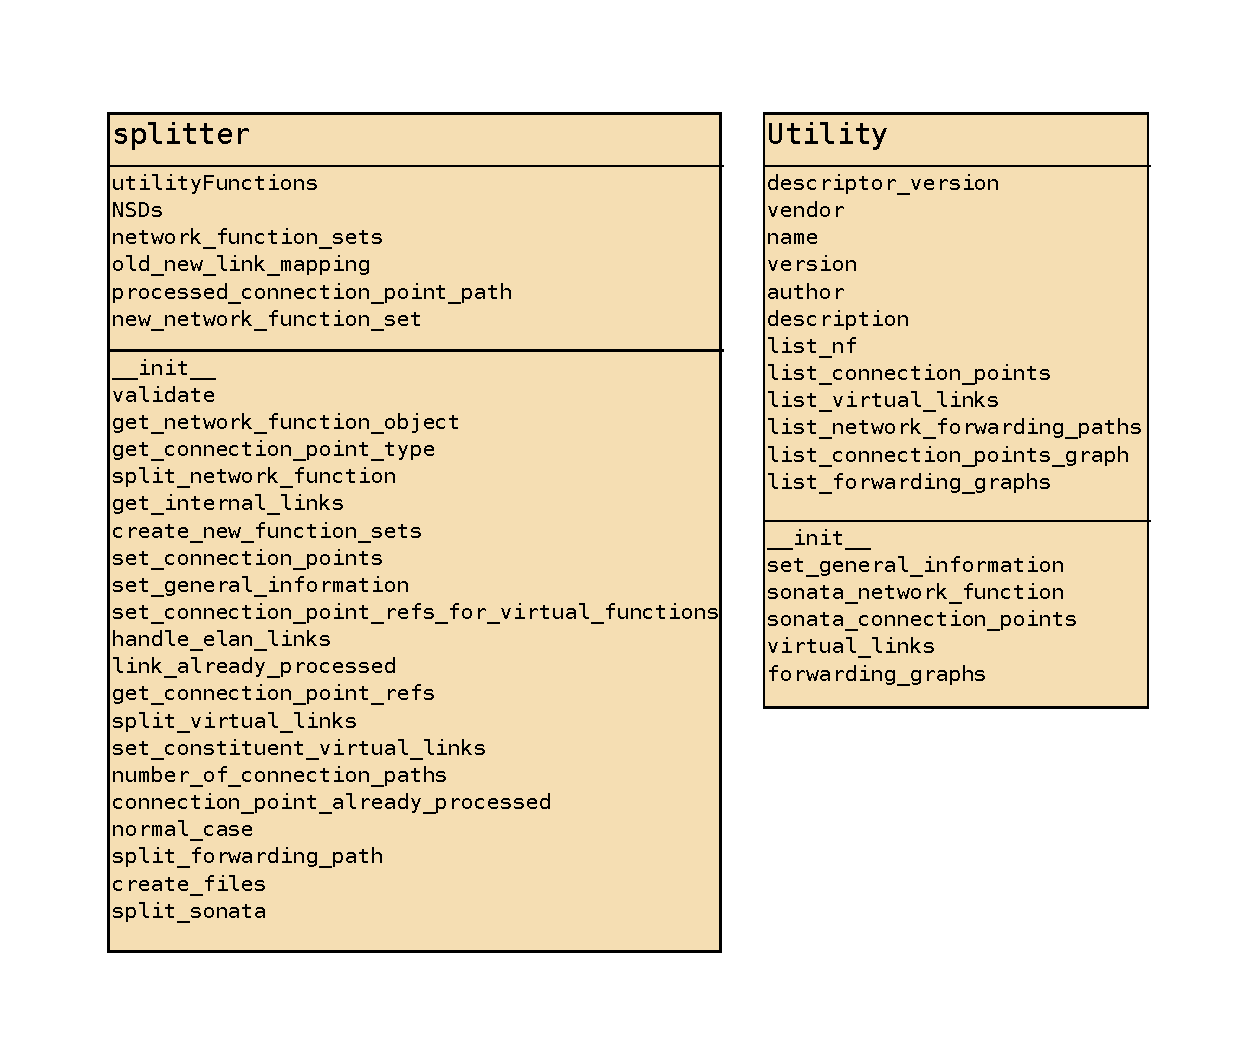
\includegraphics[width=1\linewidth]{figures/Pishahang-Splitter}
	\caption{Pishahang Splitter Class diagram}
	\label{fig:pishahangsplitterclassdiagram}
\end{figure}

\begin{figure}
	\centering
	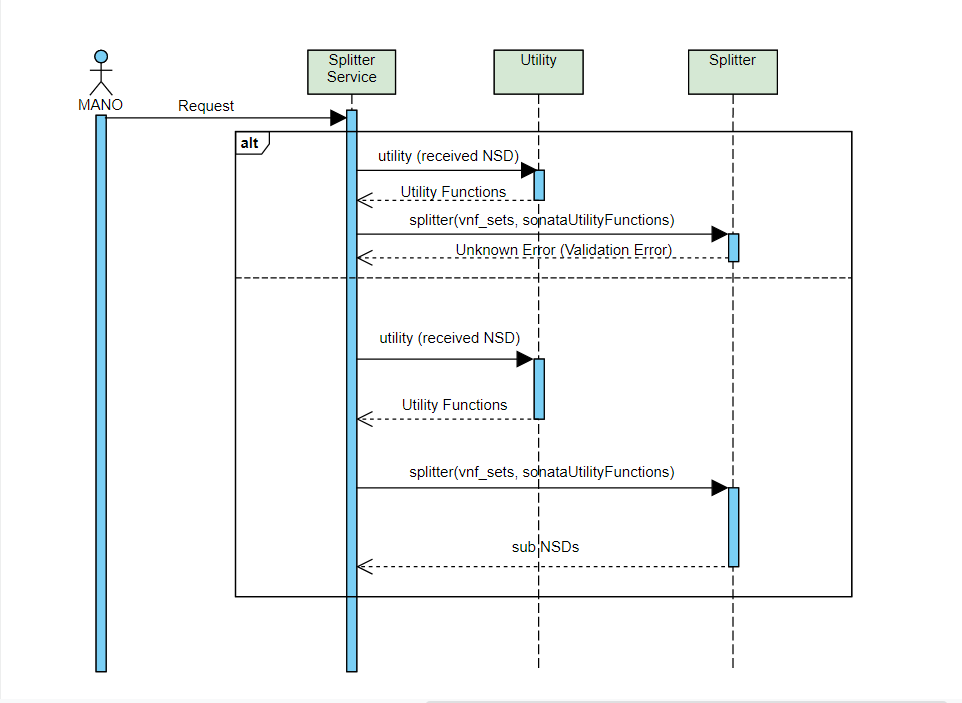
\includegraphics[width=1\linewidth]{figures/splitter_sequence_diagram}
	\caption{Splitter Sequence diagram}
	\label{fig:splittersequencediagram}
\end{figure}



\subsection{Usage}

SDS is implemented as a micro-service which can be used independently from Translator or Wrapper by making a post call to the SDS. Following code snippet describes how to call SDS using POST call.

\begin{lstlisting}[caption=POST call to SDS, label=lis:postSDS]

splitter_url=http://$HOST:8003/Main_splitter/split

# Body: descriptor contains NSD, vnfid_set contains set of VNF ids
nsd = { 'descriptor' : descriptor, 'sets': vnfid_set}

LOG.info("Calling Scramble Splitter..." )
response  = requests.post(splitter_url,
data=json.dumps(nsd_to_split))

print(response)

\end{lstlisting}

Following are some of the important functions which helps SDS in splitting the NSD with respective code snippet.

\subsubsection{Python Base classes for NSD Schema} Following code snippet shows how NSD schema is mapped to various Python classes.

\begin{lstlisting}[caption=Python Base classes, label=lis:schemaclasses]

class NetworkFunction:  # class representing a network function and its properties
    vnf_id = ""
    vnf_name = ""
    vnf_vendor = ""
    vnf_version = ""
    connection_point_refs = []

    def __init__(self, vnf_id, vnf_vendor, vnf_name, vnf_version, connection_point_refs):
        self.vnf_id = vnf_id
        self.vnf_vendor = vnf_vendor
        self.vnf_name = vnf_name
        self.vnf_version = vnf_version
        self.connection_point_refs = connection_point_refs


class ConnectionPoint:  # class representing a connection point and its properties
    _id = ""
    interface = ""
    _type = ""

    def __init__(self, _id, interface, _type):
        self._id = _id
        self.interface = interface
        self._type = _type


class VirtualLink:  # class representing a virtual link and its properties
    _id = ""
    # connectivity type can be 'E-LAN' representing many to many connectivity or
    # 'E-Line' representing one to one
    connectivity_type = ""
    connection_points_reference = []

    def __init__(self, _id, connectivity_type, connection_points_reference):
        self._id = _id
        self.connectivity_type = connectivity_type
        self.connection_points_reference = connection_points_reference

\end{lstlisting}

\subsubsection{Splitting} "split sonata" calls the splitting function one by one to split the list of objects created out of NSD. Following code snippet shows the sequence of function calls.

\begin{lstlisting}[caption=Sequence of function calls, label=lis:functioncalls]

def split_sonata(self):
if self.validate() is not False:
self.create_new_function_sets()
self.set_connection_point_refs_for_virtual_functions()
self.split_network_function()
self.set_connection_points()
self.split_virtual_links()
self.split_forwarding_path()
self.set_general_information()
return self.create_files()
else:
print("Validation Failed!!")

\end{lstlisting}

\subsubsection{Validate} Validate method validates the request coming from the MANOs. For example, if MANO is requesting a NSD to be split into three parts but the original NSD contains just two VNFs then the SDS will throw validation error.

\begin{lstlisting}[caption=Splitting Request Validation, label=lis:validation]

def validate(self):
size = 0
list_network_function = []
for network_function_set in self.network_function_sets:
size = size + len(network_function_set)
for network_function in network_function_set:
list_network_function.append(network_function)

if size != len(self.utilityFunctions.list_nf):
return False
if len(list_network_function) != len(set(list_network_function)):
return False

\end{lstlisting}

\subsubsection{Split Network Functions}
This function updates the sub NSDs with set of network functions and there properties provided in the request.

\begin{lstlisting}[caption=Network Function Splitting, label=lis:NFSplitting]

def split_network_function(self):

for network_function_set in self.network_function_sets:

sub_nsd = SonataSchema.NSD("", "", "", "", "", "", [], [], [], [])

network_function_list = []

for network_function in network_function_set:

network_function_list.append(self.get_network_function_object(network_function))

sub_nsd.networkFunctions = network_function_list

self.NSDs.append(sub_nsd)

\end{lstlisting}

\subsubsection{Split Forwarding Graph} \label{fgsplitting}
The current implementation of splitter can successfully split a NSD with three or less VNFs.To maintain the topology of the main NSD, the graph has to consider the virtual links between VNFs present in the main NSD. The main challenge in splitting a forwarding graph is to maintain the topology. In case of four or more VNFs, the possible scenarios for splitting increases which increases the complexity of splitter. It can be achieved by maintaining a mapping of original one to one virtual links while processing the virtual links and then creating new virtual link set based on the request from MANO. Example, consider three VNFs, A, B and C. Packet is supposed to flow from A to B to C. After splitting, the sequence of packet flow should not be altered. If there is a request from MANO to split the NSD into two parts with [A, C] and [B], then to insure the topology is not changed, the NSD has to be splitted into three NSDs instead of two. In reference to the above example and following code snippet, normal scenario refers to when the request from MANO is to split it in such a way which does not result in creation of new virtual links which are not there in the original NSD. 

\begin{lstlisting}[caption=Forwarding Graph Splitting, label=lis:FGSplitting]

"""
    Method splits the forwarding path.
    """
    def split_forwarding_path(self):
        for i in range(len(self.NSDs)):
            nsd_fg = self.NSDs[i]
            del self.processed_connection_point_path[:]
            for fg in self.utilityFunctions.list_forwarding_graphs:
                
                fg_inner = SonataSchema.ForwardingGraphs(fg.fg_id, fg.number_of_endpoints,
                                               len(self.set_constituent_virtual_links(nsd_fg, fg)), self.network_function_sets[i],
                                               self.set_constituent_virtual_links(nsd_fg, fg), [])
                for path in fg.network_forwarding_path:
                    if self.number_of_connection_paths(self.set_constituent_virtual_links(nsd_fg, fg)) > 1:
                        for j in range(self.number_of_connection_paths(self.set_constituent_virtual_links(nsd_fg, fg))):
                            path_inner = SonataSchema.NetworkForwardingPaths(path.fp_id + "_" + str(j), path.policy, [])
                            x = 0
                            for cp in path.connection_points:
                                if self.connection_point_already_processed(cp.connection_point_ref) is False:
                                    found = 0
                                    if cp.connection_point_ref in self.get_connection_point_refs(nsd_fg.networkFunctions):
                                        x = x + 1
                                        point = SonataSchema.ConnectionPointsGraph(cp.connection_point_ref, x)
                                        path_inner.connection_points.append(point)
                                        found = 1
                                        self.processed_connection_point_path.append([cp.connection_point_ref, 1])
                                    else:
                                        for connection_point in nsd_fg.connectionPoints:
                                            if cp.connection_point_ref == connection_point._id:
                                                x = x + 1
                                                point = SonataSchema.ConnectionPointsGraph(cp.connection_point_ref, x)
                                                path_inner.connection_points.append(point)
                                                found = 1
                                                self.processed_connection_point_path.append([cp.connection_point_ref, 1])
                                    if found == 0:
                                        string = cp.connection_point_ref.split(":")
                                        if string[1] == "input":
                                            x = x + 1
                                            point = SonataSchema.ConnectionPointsGraph("output", x)
                                            path_inner.connection_points.append(point)
                                            self.processed_connection_point_path.append([cp.connection_point_ref, 1])
                                            break
                                        if string[1] == "output":
                                            x = 1
                                            point = SonataSchema.ConnectionPointsGraph("input", x)
                                            path_inner.connection_points.append(point)
                                            self.processed_connection_point_path.append([cp.connection_point_ref, 1])
                            fg_inner.network_forwarding_path.append(path_inner)
                    else:
                        fg_inner.network_forwarding_path.append(self.normal_case(path, nsd_fg))
                nsd_fg.forwardingGraphs.append(fg_inner)
            self.NSDs[i] = nsd_fg

\end{lstlisting}

\subsection{Challenges}
The NSD schema of Pishahang and OSM contains a lot of elements. However the challenge we faced was choosing which elements to include for splitting. We tackled it by including mandatory elements and few optional elements from the schema which were present in the input NSD.
\subsection{Future scope of Service Descriptor Splitter}
SDS can currently split NSD of Pishahang and OSM. SDS is built in such a way that it can be implemented for new MANO frameworks as well. To implement SDS for a new MANO framework one can refer the implementation of either Pishahang or OSM. First step would be to create basic python classes from the NSD schema of the MANO framework then writing the utility functions to pull the information from the NSD file and store it in the objects of the basic python classes. Lastly writing splitting functions to actually split the list of objects in two or more parts.

Also, the current implementation considers all mandatory elements and a few optional elements from a NSD schema for splitting which can be extended to include other fields (Provided they are present in the input NSD for splitting).

Current implementation of SDS can split a forwarding graph of a NSD (Pishahang) with just three VNFs. Splitting of a forwarding graph is implemented by keeping future implementation for more than three VNFs in mind. (\ref{fgsplitting})


\section{Adaptor}

Facilitating easy communication between MANOs is an important aspect of scramble. 
Adaptor is a component that enables communication between MANOs by wrapping the REST APIs of MANOs in python code.\\

Python MANO Wrappers (PMW) is a uniform python wrapper library for various implementations of NFV Management and Network Orchestration (MANO) REST APIs. 
PMW is intended to ease the communication between python and MANO by providing a unified, convenient and standards oriented access to MANO API.\\

To achieve this, PMW follows the conventions from the ETSI GS NFV-SOL 005 (SOL005) RESTful protocols specification. 
This makes it easy to follow and the developers can use similar processes when communicating with a variety of MANO implementations.\\

PMW is easy to install, use and well documented. 
Code usage examples are available along with the detailed documentation at the following link \url{https://python-mano-wrappers.readthedocs.io/en/adaptor/}. \\

PMW is planned and released as an independent library. 
In scramble, PWM helps in inter communication of different instances of MANO, thereby creating opportunity for more advanced feature set, for example, hierarchical scaling. 
Operations such as on-boarding of NSD and VNFD, instantiation and termination of NS can be performed with ease.

\subsection{Architecture \& Work flow}
Standards based approach is a fundamental design principle behind PMW's design. 
A Common interface template is defined in compliance with SOL005 which contains the blueprint for all the methods mentioned in the standards. 
These methods are divided into different sections as per SOL005 into the following:

\begin{itemize}
	\item \textbf{auth: }Authorization API
	\item \textbf{nsd: }NSD Management API
	\item \textbf{nsfm: }NS Fault Management API
	\item \textbf{nslcm: }Lifecycle Management API
	\item \textbf{nspm: }NS Performance Management API
	\item \textbf{vnfpkgm: }VNF Package Management API
\end{itemize} 

In the figure \ref{fig:wrapperarch}, different sections of PMW are visualized. 
As part of the scramble project, support for Open Source MANO (OSM) and Sonata was implemented based on the common interface. 
This is represented by the dotted lines to OSM and Sonata modules. 
These modules are based on the common interface and implement the methods it has defined. 
Wrappers also support additional functionalities of Pishahang, which is an extension of Sonata. 

\begin{figure}
	\centering
	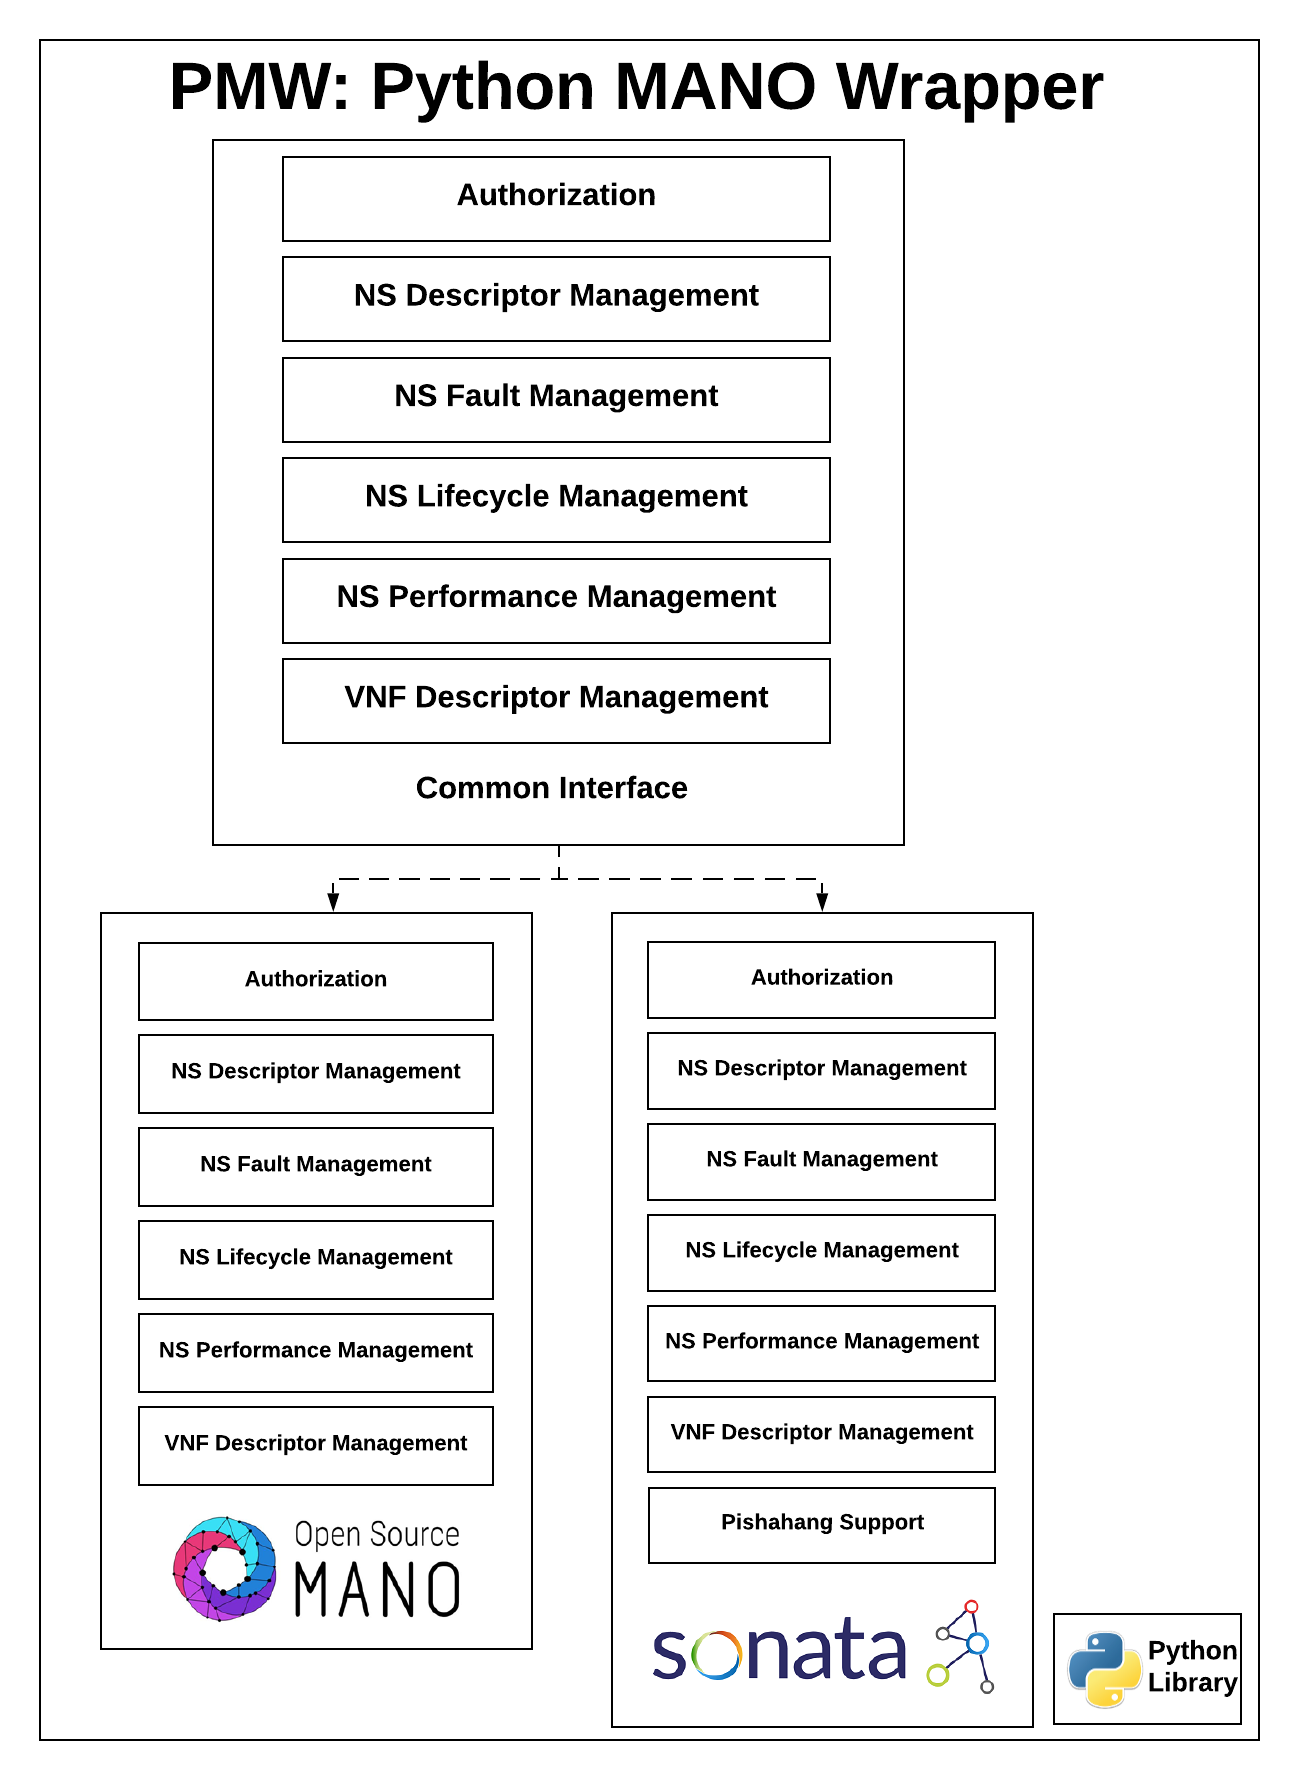
\includegraphics[width=1\linewidth]{figures/WrapperArch}
	\caption{PWM Common interfaces}
	\label{fig:wrapperarch}
\end{figure}

\begin{figure}
	\centering
	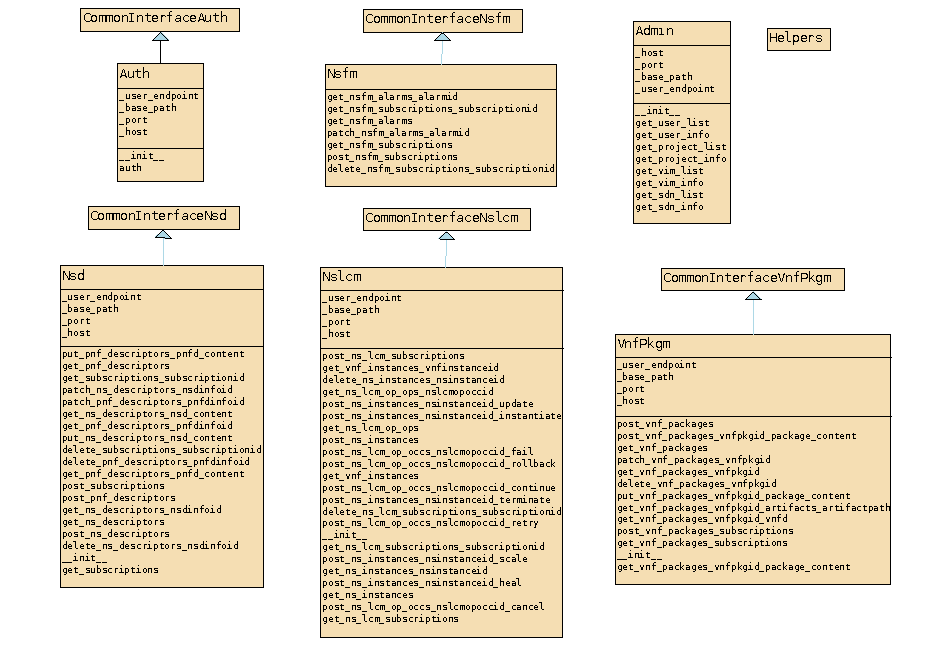
\includegraphics[width=1\linewidth]{figures/osm_class_diagram}
	\caption{OSM Wrappers implemented based on the CommonInterface base classes}
	\label{fig:osmclassdiagram}
\end{figure}

\begin{figure}
	\centering
	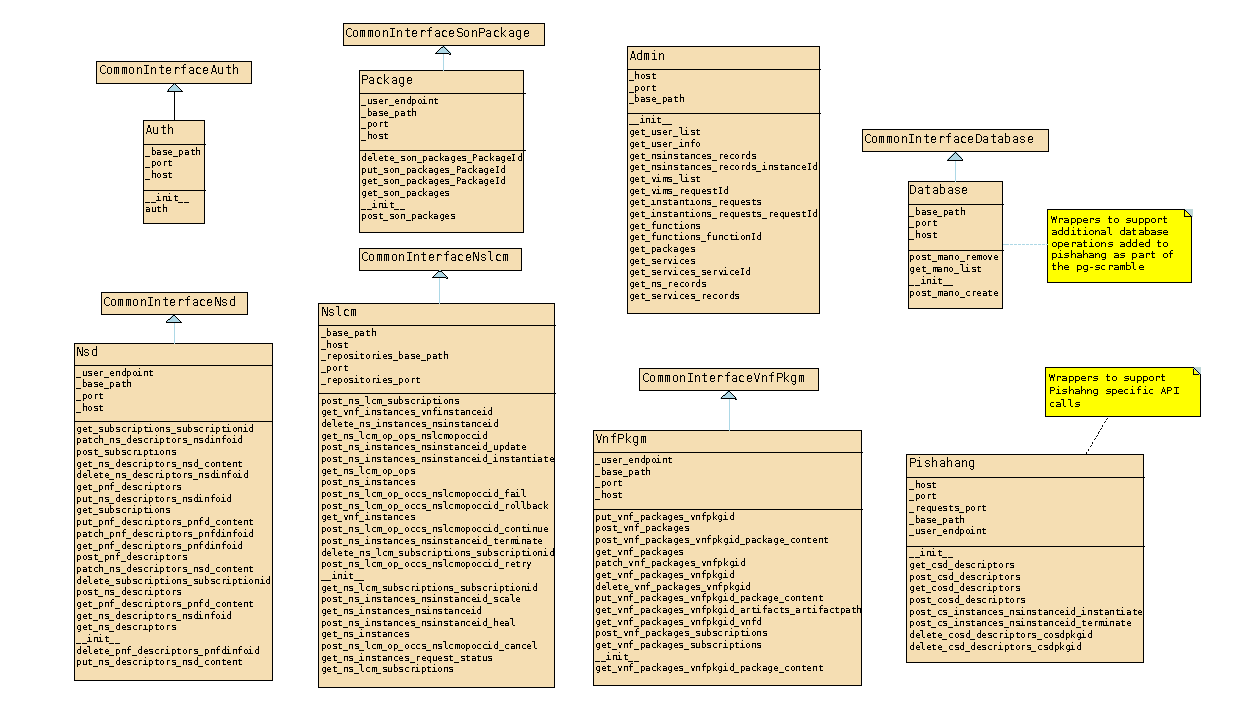
\includegraphics[width=1\linewidth]{figures/pishahang_class_diagram}
	\caption{Pishahang Wrappers implemented based on the CommonInterface base classes}
	\label{fig:osmclassdiagram}
\end{figure}


\subsection{Installation and usage}

PWM can be installed using pip by using this command \texttt{pip install python-mano-wrappers}. 

A simple script to get started with PWM is shown in the Listing \ref{lis:simpleauth}, here, the wrappers are imported and a client object is created according to the MANO type. 
Currently supported are OSM and Sonata. 
Such a client object can be used to make REST calls relevant to the MANO type. 
An example usage to retrieve all the network service descriptors of OSM can be seen from the listing \ref{lis:osmnsd}, here, the OSMClient module is used to first fetch an auth token and further using the auth token to fetch the relevant information, in this case NSD descriptors.


\begin{lstlisting}[caption=Simple wrapper code to fetch token, label=lis:simpleauth]
import wrappers

username = "admin"
password = "admin"
mano = "osm"
# mano = "sonata"
host = "osmmanodemo.com"

if mano == "osm":
	_client = wrappers.OSMClient.Auth(host)
elif mano == "sonata":
	_client = wrappers.SONATAClient.Auth(host)

response = _client.auth(
							username=username, password=password)

print(response)

\end{lstlisting}

\begin{lstlisting}[caption=Code to fetch all NSDs in OSM, label=lis:osmnsd]
import wrappers

osm_nsd = wrappers.OSMClient.Nsd(HOST_URL)
osm_auth = wrappers.OSMClient.Auth(HOST_URL)

_token = json.loads(osm_auth.auth(
									username=USERNAME,
									password=PASSWORD))

_token = json.loads(_token["data"])

response = json.loads(osm_nsd.get_ns_descriptors(
											token=_token["id"]))
response = json.loads(response["data"])
\end{lstlisting}

\subsection{Challenges}

Implementing such a python wrapper for a REST API is straight forward from the implementation perspective. 
However, the challenges that we faced are when identifying the required functional documentation from the respective MANOs. 
OSM and Sonata do not yet fully support the ETSI suggested endpoints and this combined with the lack of unified documentation, made it difficult in the begining to decide on the scope of supported functionalities.\\
  

\subsection{Future scope of wrappers}

PWM is built with easy maintanability and feature addition in mind. 
PWM makes it easy to add support for other MANOs. 
We expect MANO developers to use the common interface that we have suggested to add support to their REST APIs in python.

 


\section{Pishahang-Scramble Integration}

Service Life-cycle Management(SLM) component of Pishahang carries out the main task of orchestration. As a result it was all the more relevant to add one more aspect to it for integrating and handling Scramble components.

The main class of SLM, \textit{ServiceLifecycleManager}, contains a list of member functions for carrying out the entire orchestration. One of the many member functions, \textit{SLM\_mapping}, is responsible for handling the descriptors payload and creating a mapping of network functions to the available VIMs. Keeping the original flow of SLM intact, we extended the main class to include a new member function (\textit{SLM\_mapping\_scramble}) to handle request addressed for mapping the network functions to the available MANOs.

When a request to instantiate the network service from the BSS (son-bss) is made, the gatekeeper (son-gkeeper) gets the request payload from BSS and creates a instantiation request to hand it over to SLM. For differentiating the instantiation request between a "\textit{normal}" call and a "\textit{scramble}" call, we added a "\textit{scramble}" button in BSS. 

\begin{lstlisting}[caption=BSS instantiateScramble function, label=lis:BSSscramble]
instantiateScramble:function(id, ingresses, egresses, ENV, selectedmanos, manodetails){				
var defer=$q.defer();

{...} ## unchanged

var data={"service_uuid":id, "ingresses": ingresses, "egresses": egresses, "scramble":true, "selectedmanos":selectedmanos, "manoips":manodetails};
$http.post(ENV.apiEndpoint+"/requests",data)
.then(function successCallback(result){defer.resolve(result)})
.catch(function errorCallback(error){defer.reject(error)});

return defer.promise;
},

\end{lstlisting}

This function sends the gatekeeper a payload which consists of a token "\textit{scramble}", which set to true, and a list of MANO details.

The gatekeeper also ensures the payload contains this additional package when it creates a new instantiation request and informs the SLM. 

\begin{lstlisting}[caption=create instantiation request in gatekeeper(request.rb), label=lis:request.rb]

post '/requests/?' do
log_msg = MODULE + '::POST /requests'
original_body = request.body.read
logger.debug(log_msg) {"entered with original_body=#{original_body}"}
params = JSON.parse(original_body, quirks_mode: true)
logger.debug(log_msg) {"with params=#{params}"}

# we're not storing egresses or ingresses
egresses = params.delete 'egresses' if params['egresses']
ingresses = params.delete 'ingresses' if params['ingresses']
user_data = params.delete 'user_data' if params['user_data']

begin
{...} ## unchanged

if params['scramble'] == true
start_request['scramble'] = true 
start_request['selectedmanos'] = params['selectedmanos']
start_request['manoips'] = params['manoips']

end
{...} ## unchanged
end

\end{lstlisting}

\begin{figure}[H]
	\centering
	\includegraphics[width=1\linewidth]{"figures/scramble_seq_diag"}
	\caption{Integration sequence diagram}
	\label{fig:sequence-diagram-scramble}
\end{figure}

\subsection{SLM\_mapping\_scramble}

This member function, together with four other helper functions, is responsible for treating requests routed for translation, splitting and sending the descriptor for instantiating in other MANOs. The 4 other helper functions used by it are as follows:
\begin{table}[H]
	\begin{center}
		\caption{Helper functions.}
		\label{tab:table2}
		\begin{tabular}{l|l} 
			\textbf{Functions} & \textbf{Description} \\
			\hline\\
			\textbf{get\_network\_functions} & \makecell[l]{It gets the network function names and ids from \\ the service descriptor.} \\\\
			\textbf{random\_combination} & \makecell[l]{It maps different network functions to different \\ MANOs in random combination.}  \\\\
			\textbf{send\_to\_osm} & \makecell[l]{This function sends one part of the splitted \\ service descriptor and its network functions to \\OSM Mano instance.} \\\\
			\textbf{send\_to\_pishahang} & \makecell[l]{This function sends one part of the splitted \\ service descriptor and its network functions to \\ PISHAHANG Mano instance.}\\\\
			\textbf{inform\_gk\_instantiation\_scramble} & \makecell[l]{This function is used to inform the gatekeeper to \\ create a dummy NSR in the only case when none \\ of the network functions, of the original NSD, are \\ instantiated by this SLM. This way the instantiation \\ request is not rolledback}
		\end{tabular}
	\end{center}
\end{table}

This function is created by extending the original \textbf{SLM\_mapping} function to include the logic to map each network functions to a MANO and then send and instantiate them in their mapped MANOs:

\begin{lstlisting}[language=Python,caption=Extended \textbf{SLM\_mapping\_scramble} function, label=lis:SLM_scramble]
def SLM_mapping_scramble(self, serv_id):
"""
This method is used if the SLM is responsible for the placement.
:param serv_id: The instance uuid of the service
"""
corr_id = str(uuid.uuid4())
self.services[serv_id]['act_corr_id'] = corr_id

LOG.info("Service " + serv_id + ": Calculating the placement ")
topology = self.services[serv_id]['infrastructure']['topology']

## getting all manos information from payload
mano_dict = self.services[serv_id]['payload']['selectedmanos']
mano_details = self.services[serv_id]['payload']['manoips']
mano_list = []

## creating a list of selected manos and its corresponding details
for key, val in mano_dict.items():
for manos in mano_details:
if manos['name']==key and val == True:
mano_list.append(manos)

## original flow with scramble portion added
if 'nsd' in self.services[serv_id]['service']:

descriptor = self.services[serv_id]['service']['nsd']
functions = self.services[serv_id]['function']
original_nsd_uuid = descriptor['uuid']

##----------------------------------------------------------------##
##----------------------SCRAMBLE PART-----------------------------##
##----------------------------------------------------------------##

# create a set of vnfs for different MANO frameworks through random logic
# Number of splits is by default 2 except if the number of MANOs and number of VNFs are equal.

function_list = self.get_network_functions(descriptor)
rndm_sets = self.random_combination(function_list, mano_list)

if(len(rndm_sets) > 1): # if there are more than 1 MANOs, SCRAMBLE-splitter is called to split the NSD
vnfid_set = [sets[0] for sets in rndm_sets]# vnf-ids of sets 1 and 2

# send the random vnf split to SCRAMBLE Splitter and get back sub NSDs for each split.
splitter_url = os.environ['splitter_url'] 
nsd_to_split = { 'descriptor' : descriptor, 'sets': vnfid_set}

response  = requests.post(splitter_url,
data=json.dumps(nsd_to_split))

nsds_splitted = json.loads(response.text) # get back 2 sets of sub-nsds

else:

nsds_splitted = {"message" : [descriptor]}


# logic to check which vnf is to be send to which MANO

function_pish = [] # list to store vnfs for MAIN_PISHAHANG
main_pish_nsd = {} # string to store nsd for MAIN_PISHAHANG

for i,sets in enumerate(rndm_sets):

if sets[2][0]['type'] == 'MAIN_PISHAHANG':

main_pish_nsd = nsds_splitted['message'][i]

for vnf in functions:
if(vnf['vnfd']['name'] in sets[1]):
function_pish.append(vnf)


elif sets[2][0]['type'] == 'PISHAHANG':

self.send_to_pishahang(serv_id, sets, functions, nsds_splitted['message'][i])

elif sets[2][0]['type'] == 'OSM':

self.send_to_osm(serv_id, sets, functions, nsds_splitted['message'][i])             

# remove the vnfs which are sent to other MANO from self.services[serv_id]['function']
NSD = main_pish_nsd
functions = function_pish
NSD['uuid'] = original_nsd_uuid

self.services[serv_id]['service']['nsd'] = NSD
self.services[serv_id]['function'] = functions

if(functions == []):

## put up a dummy nsr when there is no network functions is available for this mano. So as to keep the unique UUID of this instantiation request in ledger instead of forced rollback.

self.inform_gk_instantiation_scramble(serv_id)

else:
content = {'nsd': NSD,
'functions': functions,
'topology': topology,
'serv_id': serv_id} 
else:
{...} ## unchanged
\end{lstlisting}



\section{Installation of Pishahang with Scramble}

In order to use and exploit the functionalities of all the work packages of scramble described above, additional steps needs to be executed after a clean installation of Pishahang. The steps are listed below in the script.
\begin{lstlisting}[caption= install Pishahang with scramble, label=lis:Pishahang_scramble]
sudo apt-get install -y software-properties-common
sudo apt-add-repository -y ppa:ansible/ansible
sudo apt-get update
sudo apt-get install -y ansible
sudo apt-get install -y git
git clone --single-branch --branch scramble-pishahang https://github.com/CN-UPB/pg-scrambLe.git
cd pg-scrambLe/phishahang/Pishahang-master/son-install

git checkout install-pishahang
mkdir ~/.ssh
echo sonata | tee ~/.ssh/.vault_pass

ansible-playbook utils/deploy/sp.yml -e "target=localhost public_ip=<<ip-address>>" -v

cd pg-scrambLe
sudo ./run_scramble.sh <<ip-address>>

\end{lstlisting}

\section{Scramble GUI for Pishahang}
The scramble-gui is integrated with both pishahang-gui and in pishahang-BSS developed with Angular-js for front end and mangodb deployed using python for back-end., enabling users to enter the details of child-MANO's and also select the desired MANO's to instantiate a service.

With Scramble-pishahang GUI the users can enter details of child-MANO's as shown in images below.

Step 1: Select \textit{MANO Settings} and then \textit{Add MANO}
\begin{figure}[H]
	\centering
	\includegraphics[width=1\linewidth]{"figures/son-gui-step-1"}
	\caption{Scramble\_pishahang GUI}
	\label{fig:sequence-diagram-scramble}
\end{figure}

Step 2: Enter MANO details, The required MANO details are 
\begin{enumerate}
	\item MANO Name: The name is take so that the user can easily differentiate between MANO's and can be any name desired by user.
	\item URL: Is the URL to access the MANO
	\item Username and Password: Is the credentials required to access the MANO
	\item MANO Vendor: Is a choice between OSM and Pishahang to recognize the type of child-mano added.   
\end{enumerate}
\begin{figure}[H]
	\centering
	\includegraphics[width=1\linewidth]{"figures/son-gui-step-2"}
	\caption{Scramble\_pishahang GUI}
	\label{fig:sequence-diagram-scramble}
\end{figure}

Once the MANO details are entered and the list of MANO's added are displayed.
\begin{figure}[H]
	\centering
	\includegraphics[width=1\linewidth]{"figures/son-gui-step-3"}
	\caption{Scramble\_pishahang GUI}
	\label{fig:sequence-diagram-scramble}
\end{figure}

Once the child-MANO's are added, in the pishahang-bss the added MANO's are listed. The user can select the MANO's in which the service can be instantiated and also if user does not need to instantiate the service in child MANO, he can instantiate the service just in the parent MANO as shown below.
\begin{figure}[H]
	\centering
	\includegraphics[width=1\linewidth]{"figures/son-bss"}
	\caption{Scramble\_pishahang GUI}
	\label{fig:sequence-diagram-scramble}
\end{figure}
  